\makeatletter
\def\input@path{{./tex/acmart/}}
\makeatother


\documentclass[
  acmsmall,
  screen,
  review,      % remove this for camera-ready
  anonymous,   % remove for camera-ready
  nonacm       % PACMPL papers use PACMPL style but are technically non-ACM proceedings submissions
]{acmart} 

% --- metadata ---
\title{A Formalization of Abstract Rewriting}

\author{Samuel Arkle}
\affiliation{
  \institution{Appalachian State University}
  \country{USA}
}
\email{arklesd@appstate.edu}

\author{Andrew Polonsky}
\affiliation{
  \institution{Appalachian State University}
  \country{USA}
}
\email{polonskya@appstate.edu}

% --- Keywords, CCS ---
\keywords{Abstract rewriting, Formalization, Confluence, Strong normalization, Newman's Lemma, Well-foundedness}

% \begin{CCSXML}
% <ccs2012>
%    <concept>
%       <concept_id>10003752.10003790.10011741</concept_id>
%       <concept_desc>Theory of computation~Type theory</concept_desc>
%       <concept_significance>300</concept_significance>
%    </concept>
% </ccs2012>
% \end{CCSXML}

\ccsdesc[300]{Theory of computation~Type theory}

% --- packages & macros ---
\usepackage{hyperref}
% \usepackage{tikz}
\usepackage{amsmath}
\usepackage{amsthm}
\usepackage{pifont}
\usepackage{mathrsfs}
\usepackage{amssymb}
\usepackage{xcolor}
\usepackage{colortbl}
\usepackage{tikz-cd}
\usepackage{caption}
\usepackage{newunicodechar}


\usepackage[utf8]{inputenc}
\usepackage{ucs}
% \DeclareUnicodeCharacter{03A3}{\ensuremath{\Sigma}}



\usetikzlibrary{positioning,shapes.geometric,fit,arrows.meta}


\captionsetup{justification=centering}



\definecolor{darkgreen}{rgb}{0.0, 0.5, 0.0}

\newcommand{\tto}{\twoheadrightarrow}
\newcommand{\sse}{\subseteq}
\newcommand{\bset}{\mathbf{Set}}
\newcommand{\nat}{\mathbb{N}}

% Comments
\newcommand{\sacomment}[1]{\textcolor{green}{#1}}
\newcommand{\apcomment}[1]{\textcolor{blue}{#1}}
\newcommand{\greyout}[1]{\textcolor{gray}{#1}}
\newcommand{\err}[1]{\textcolor{red}{#1}}

% Theorem style
% \newtheorem{thm}{Theorem}
% \newtheorem{dfn}[thm]{Definition}
% \newtheorem{prop}[thm]{Proposition}
% \newtheorem{cor}[thm]{Corollary}
% % \newtheorem{lemma}[thm]{Lemma}
% % \newtheorem{rmk}[thm]{Remark}
% % \newtheorem{expl}[thm]{Example}
% \newtheorem{notn}[thm]{Notation}
% %\theoremstyle{nonumberplain}
% %\theoremsymbol{\Box}
% % \newtheorem{proof}{Proof}

\newcommand{\RP}{\mathrm{RP}}
\newcommand{\gRP}{\mathbf{RP}}
\newcommand{\RPm}{\mathrm{RP^{-}}}
\newcommand{\gRPm}{\mathbf{RP^{-}}}
\newcommand{\NF}{\mathrm{NF}}
\newcommand{\MF}{\mathrm{MF}}
\newcommand{\UN}{\mathrm{UN}}
\newcommand{\gUN}{\mathbf{UN}}
\newcommand{\UNto}{\mathrm{UN}^{\to}}
\newcommand{\gUNto}{\mathbf{UN}^{\to}}
\newcommand{\SN}{\mathrm{SN}}
\newcommand{\gSN}{\mathbf{SN}}
\newcommand{\decSN}{\mathrm{dec(SN)}}
\newcommand{\SM}{\mathrm{SM}}
\newcommand{\SMseq}{\mathrm{SMseq}}
\newcommand{\gSMseq}{\mathbf{SMseq}}
\newcommand{\gSM}{\mathbf{SM}}
\newcommand{\WN}{\mathrm{WN}}
\newcommand{\gWN}{\mathbf{WN}}
\newcommand{\SMandWN}{\mathrm{SM\land WN}}
\newcommand{\gSMandWN}{\mathbf{SM\land WN}}
\newcommand{\WM}{\mathrm{WM}}
\newcommand{\gWM}{\mathbf{WM}}
\newcommand{\WNFP}{\mathrm{WNFP}}
\newcommand{\NP}{\mathrm{NP}}
\newcommand{\gNP}{\mathbf{NP}}
\newcommand{\NPe}{\mathrm{NP_=}}
\newcommand{\gNPe}{\mathbf{NP_=}}
\newcommand{\WMFP}{\mathrm{WMFP}}
\newcommand{\MP}{\mathrm{MP}}
\newcommand{\gMP}{\mathbf{MP}}
\newcommand{\CR}{\mathrm{CR}}
\newcommand{\CRs}{\mathrm{CR^{\le 1}}}
\newcommand{\gCRs}{\mathbf{CR^{\le 1}}}
\newcommand{\gCR}{\mathbf{CR}}
\newcommand{\WCR}{\mathrm{WCR}}
\newcommand{\gWCR}{\mathbf{WCR}}
\newcommand{\Inc}{\mathrm{Inc}}
\newcommand{\gInc}{\mathbf{Inc}}
% \newcommand{\BP}{\mathrm{BP}}
\newcommand{\gBP}{\mathbf{BP}}
\newcommand{\FB}{\mathrm{FB}}
\newcommand{\CP}{\mathrm{CP}}
\newcommand{\gCP}{\mathbf{CP}}



\newcommand{\from}{\leftarrow}



\newcommand{\red}[1]{\textcolor{red}{#1}}
\newcommand{\blue}[1]{\textcolor{blue}{#1}}

% Reduction relation macros
\newcommand{\rstep}{\mathbin{\longrightarrow_R}}
\newcommand{\mstep}{\mathbin{\longrightarrow_R^*}}
\newcommand{\estep}{\mathbin{\longrightarrow_R^=}}
\newcommand{\rrstep}{\mathbin{\longrightarrow_R^r}}
\newcommand{\brstep}{\mathbin{\longleftarrow_R^r}}
\newcommand{\bstep}{\mathbin{\longleftarrow_R}}
\newcommand{\bmstep}{\mathbin{\longleftarrow_R^*}}

% Unicode characters

\newunicodechar{∀}{\ensuremath{\forall}}
\newunicodechar{→}{\ensuremath{\rightarrow}}
\newunicodechar{ℕ}{\ensuremath{\mathbb{N}}}
\newunicodechar{↔}{\ensuremath{\leftrightarrow}}
\newunicodechar{⊆}{\ensuremath{\sse}}
\newunicodechar{∧}{\ensuremath{\land}}
\newunicodechar{₌}{\ensuremath{_=}}
\newunicodechar{𝓟}{\ensuremath{\mathcal{P}}}
\newunicodechar{∈}{\ensuremath{\in}}
\newunicodechar{φ}{\ensuremath{\phi}}
\newunicodechar{Σ}{\ensuremath{\Sigma}}
\newunicodechar{₁}{\ensuremath{{}_1}}


% Misc Macros
\newcommand{\terese}{[TeReSe]}
% \newcommand{\ul}[1]{\underline{#1}}
\newcommand{\ule}[1]{\underline{#1:}}
% \newcommand{\setof}[1]{\{#1\}}
\newcommand{\setof}[1]{\left\{#1\right\}}


\newcommand{\tclos}[1]{{#1}^{\scriptscriptstyle{+}}}


% Taken from well founded section

\newcommand{\isWFacc}{\mathtt{isWFacc}}
\newcommand{\isWFseq}{\mathtt{isWFseq}}
\newcommand{\isWFmin}{\mathtt{isWFmin}}
\newcommand{\isWFaccm}{\mathtt{isWFacc-}}
\newcommand{\isWFseqm}{\mathtt{isWFseq-}}
\newcommand{\isWFminm}{\mathtt{isWFmin-}}

\newcommand{\isMinDec}{\mathtt{isMinDec}}
 
% \newtheorem{definition}{Definition}
% \newtheorem{notation}{Notation}
\newtheorem{remark}{Remark}
\theoremstyle{acmdefinition}
\newtheorem{notation}{Notation} 
% \newtheorem{notation}[theorem]{Notation} % Can't get this to work

% \supplement{https://github.com/DrPolonsky/FPLA/tree/main} %TODO: Can't get this reference to the code to work.
\usepackage{enumitem}
% --- begin document ---
\begin{document}

\begin{abstract}
    We present a constructive formalization of Abstract Reduction Systems (ARS)
    in the Agda proof assistant, focusing on the results given in the standard
reference on Term Rewriting Systems \cite{Terese}. We define a taxonomy of
concepts related to termination and confluence and investigate their
relationships between each other and their classical counterparts. We identify,
and eliminate where possible, the use of classical logic in the proofs of
standard ARS results. Our analysis leads to refinements and mild
generalizations of classical termination and confluence criteria. Finally, we
investigate logical relationships between several notions of termination,
arising from different formulations of the concept of a well-founded relation.
\end{abstract}

\maketitle

\section{Introduction}
\label{sec:Introduction}

% \section{Plan}
% \begin{itemize}
%   \item Start by discussing motivation
%   \item Then contributions
%   \item Plan of the paper
%   \item At some point, there should be like a summary of what's been done and what are some interesting discoveries
% \end{itemize}
%


We present a formalization of the basic Abstract Rewriting Systems (ARS) theory as presented in Term Rewriting Systems [TeReSe]
 \cite{Terese}, using the Agda proof assistant.
This work is part of a larger effort to develop a library of formalized programming language theory (PL)
at Appalachian State University.
Since Term Rewriting Systems (TRS) play a foundational role in programming languages,
while ARS encompass the basic facts about rewriting relations in general,
establishing these facts is part of the necessary infrastructure required to
pursue the broader project.  The present contribution can therefore be seen as
``bootstrapping'' Appalachian State's new formalized PL repository.

This broader goal also drives the main design choices in our approach.
Since rewriting theory is concerned with a fine-grained analysis of computation,
the most natural vehicle for formalizing it is type theory based on the
Curry--Howard isomorphism, which Agda implements.  Proofs in this language
are automatically effective, and implicitly carry the code that implements
a transformation from the hypotheses to the conclusion of the claim.  For example,
a type-checked proof that a given TRS is Church--Rosser automatically renders a function that
computes a common reduct between any two convertible terms.

Staying within this paradigm requires the proofs to be constructive.
Moreover, it requires us to avoid any axioms or postulates, such as function
extensionality, uniqueness of identity proofs, univalence, etc.
While most of ARS results are indeed constructive, standard presentations,
 including \cite{Terese}, make liberal use of classical logic.
Our paper can thus be read as a thoroughly constructive
development of elementary ARS theory.

\subsection{Motivation}

Before we proceed further, let us consider two formalization scenarios where
a constructive ARS library can be useful.

\begin{example}[Formalization of a typed lambda calculus]
Suppose one is formalizing the standard metatheory of
a typed lambda calculus.  To show confluence, one can
first establish the Church--Rosser theorem (CR) for the untyped lambda calculus,
and then proceed via the Subject Reduction theorem.
However, suppose that Strong Normalization had already been verified independently.
Invoking Newman's lemma, one can conclude confluence from the weak
diamond property --- which is generally easier to prove than full CR.
\end{example}

\begin{example}[Quotients of types]
Suppose one wishes to construct the initial model of an algebraic theory $T$
over a first-order signature $S$.
(For example, the reader could think here of the free commutative semiring over a finite set of generators.)
The classical definition involves the quotient of the term algebra $S^*$ by
the equivalence relation $\approx_T$ induced by $T$.
Direct encoding of quotients is problematic in pure type theory.
While there are a number of solutions, such as Higher Inductive Types \cite{HoTT},
Quotient Inductive--Inductive Types \cite{QIIT}, Cubical Type Theory \cite{CTT}, etc.,
they involve extending type theory with new language constructs,
incurring additional costs in complexity.

Now, suppose $T$ admits a convergent presentation.
That is, suppose that the equivalence relation on $S^*$ coincides
with conversion generated by a confluent and terminating rewriting system
$\to_R : S^* \to S^* \to \bset$.
Then one can replace $S^*/{\approx_T}$ by the type of $R$-normal forms.
(In the semiring example, these would be polynomial expressions sorted according to
an appropriate ordering on monomials.)
This can be defined as a pure dependent type
\[ NF(R) \quad := \quad (\Sigma n : S^*) (\Pi x : S^*) \lnot (n \to_R x) \]
This type encodes the quotient in the sense that the type of functions $S^*/{\approx_T} \to A$ is isomorphic to plain functions from $NF(R)$ to $A$.
Indeed, the elimination rule for the quotient type requires every equation in $T$
to be validated in order to define a function $f : S^*/{\approx_T} \to A$.
Any such function trivially specializes to $NF(R)$.  In the other direction,
a plain function from $NF(R)$ to $A$
can be extended to all of $S^*$ by induction on normalizing reduction sequences.
Confluence ensures that $T$-equal elements are always mapped to the same value.

It follows that $S^*/{\approx_T}$ is isomorphic to $NF(R)$.

It also follows as a corollary that equality in the initial model is decidable.
\end{example}

As these examples illustrate, a fully effective implementation of basic ARS results
can be helpful in many settings arising in programming language theory.

\subsection{Formalization principles}
With the explicit goal of having the results of basic abstract rewriting
formalized in a canonical way, so that they can be used in building
libraries of formalized PL theory, we adopted the following
principles during our development.

\begin{itemize}
  \item No use of function extensionality;
  \item No use of univalence, uniqueness of identity proofs, axiom K, or any other
  assumptions related to equality;
  \item Minimize the use of classical logic, and make decidability hypotheses explicit in every place where classical logic could not be avoided;
  \item Stay as faithful as possible to the spirit of type theory based on the Curry--Howard isomorphism, so that in every concrete application, our proofs would compute.
\end{itemize}

\subsection{Decidability}
In several places, we had to assume certain decidability hypotheses in order to make
the proofs go through.  These were always flagged explicitly, and an effort was made to
have as few of them as possible.

Recall that a relation is strongly normalizing iff its converse is well-founded. \cite[Def.1.1.13]{Terese}.
Since normalization is a central concept in ARS theory,
we pay special attention to the concept of well-foundedness.
The standard constructive definition does not even allow one to show that SN implies WN,
as we discuss in Section \ref{sec:Well-foundedness} and formalize in \texttt{WFCounters.agda} \sacomment{Should this now be ARS/Examples.agda?}.
We therefore looked at a number of variations of this notion in the constructive context,
their classical counterparts all being logically equivalent. %This gave rise to a rich set of concepts, see Figure \ref{f:wf}.

We have also identified classes of ARSs where the needed classical principles are simply valid.  In particular, for finitely branching relations, the implication SN to WN requires nothing else beyond plain decidability of the relation itself: $Rxy \lor \lnot Rxy$.  For example, an ARS induced by a first-order TRS with a finite set of rules is both finitely branching and decidable.

The main conclusion of our work is that most of the main ARS results can be made completely effective, at least for the practical examples encountered in first-order TRSs and lambda calculi.

For more exotic rewrite systems --- like $\lambda \bot$ (underpinning sensible lambda theories), or coinductive rewriting ---
these decidability assumptions no longer hold, and the utility of the ARS framework diminishes proportionally.

\subsection{Contributions and related works}
Several formalizations of the concepts of elementary ARS theory exist, including projects in Isabelle \cite{isabelleFormalization}, PVS \cite{trs}, and Rocq \cite{coqARS} as well as the Agda standard library \cite{AgdaLibraryRewriting}.
The first three are quite mature large-scale projects for certifying termination of
general rewrite systems.  Our work is more comparable in scale to the rewriting development in the
Agda library, and is meant to serve as a starting point for a new library of formalized
programming language theory.  The specific contributions we provide beyond the works cited above
are as follows.
% Our work distinguishes itself through contributions 2-5 above: the detailed ontology of termination and confluence properties, new ARS concepts, refinements to classical criteria, and  examining multiple notions of well-foundedness.
% Our contributions are as follows.
\begin{itemize} \label{list:ourContributions}
  \item An original formalization of elementary ARS theory as presented in Terese
  \cite{Terese}, including relevant background about relations and logic;
  % Chapter 1 of
  \item An ontology of termination and confluence properties, and a detailed analysis of logical relationships between them;
  \item Definitions of new ARS concepts that refine our understanding of these relationships;
  \item Marginal improvements to classical confluence and termination criteria;
  \item An examination of several distinct notions of well-foundedness
  in the constructive setting.
\end{itemize}

% \subsection{Related works}
% We should cover the following in this section:
% \begin{itemize}
%   \item The IsaFoR/CeTA tool for certification of termination/confluence proofs provided by some automated tool (http://cl-informatik.uibk.ac.at/software/ceta/#introduction). Specifically this paper (https://www.isa-afp.org/entries/Abstract-Rewriting.html) deals with the formalization of strong normalization and Neman's lemma as part of the CeTA project. They use Isabelle for their formalization.
%   \item This termination portal which gives an overview of various termination tools: https://termination-portal.org/wiki/Termination_Portal. Specifically here is a list of different termination tools: https://termination-portal.org/wiki/Category:Tools . We should talk about what distinguishes our project from a termination tool.
%   \item Similarly this project is a collection of formalizations of theorems related to term rewrite systems in the language of the proof assistant PVS. http://trs.cic.unb.br/ (here is the formalization of Newman's lemma if you're interested! https://github.com/nasa/pvslib/blob/master/TRS/newman_yokouchi.pvs).
%   \item Can nention that the agda standard library has a rewriting formalization too based on TeReSe
% \end{itemize}

\subsection{Plan of the paper}

The structure of the paper roughly corresponds with the progression of the Agda code.
% Agda files.
% (with the exception of section \ref{sec:Well-foundedness}, which is put at the end)
In the next section, we lay out the main properties of relations studied in ARS theory,
setting the ground for what follows.  In Section \ref{sec:Formalization}, we
outline our formalization of the ARS chapter from \cite{Terese}.
Here we also discuss how this effort suggested new ARS properties that helped us overcome some obstacles we encountered along the way.  These properties fit naturally within the rewriting paradigm.  Thus in Section \ref{sec:Hierarchy}, we dedicate some effort to investigating them further.  The result is a broader ontology of ARS concepts, revealing interrelationships between conditions for completeness.  In Section \ref{sec:Well-foundedness} we focus on what it means for a relation to be well-founded, identifying the classical principles needed to transition between different formulations.
We conclude with a brief summary and suggestions for future work.

\section{Definitions}
\label{sec:Definitions}
\sacomment{Need to update move from WNFP to NP, WMFP to MP, NP to NP\_0}
\sacomment{Need to update to refer to macros for properties}
The following definitions are provided to ensure clarity and precision
in our discussion.
 When useful, we also include the name and type of
definition as we have implemented it in Agda, allowing the report to guide the code
and vice versa.



\begin{definition}
    An abstract rewrite system (\emph{ARS}) is a structure $\mathcal{A} = (A, R_\alpha)$ where
     $A$ is a set of elements and $R_\alpha$ is a set of binary relations on $A$.
\end{definition}

For the rest of this section, let $A$ be a fixed set, and $R$ be a relation on $A$.
(In the Agda code supplement, this is represented by a type $A : \bset$,
and a binary type family $R : A \to A \to \bset$.)

\greyout{We denote by $\tilde R$ the relational converse of $R$ ($(x,y) \in \tilde R \iff (y,x) \in R$),
and by $R;R'$ the relational composition of $R$ and $R'$.}


\begin{notation}
  The following notions are standard.  For precise definitions,
  see \texttt{ClosureOperators.agda}.
  \begin{enumerate}
    \item $R^r$ denotes the \emph{reflexive closure} of $R$.
    \item $R^s$ denotes the \emph{symmetric closure} of $R$.
    \item $R^+$ denotes the \emph{transitive closure} of $R$.
    \item $R^* = (R^r)^+$ denotes the \emph{reflexive-transitive closure} of $R$.
    \item $R^= = (R^s)^*$ denotes the \emph{equivalence relation generated by} $R$.
  \end{enumerate}
\end{notation}




In the context of abstract rewriting, we will often write $a \rstep b$
in place of $(a,b) \in R$.  Similarly, we will write $a \mstep b$ for $(a,b) \in R^*$,
$a \bstep b$ for $(b,a) \in R$.  When the relation $R$ is clear from the context,
we may drop the corresponding subscript.

We next define rewriting-theoretic concepts like confluence and normalization relative to a fixed element of $A$; global versions of these properties are obtained by universal quantification.
For equivalent definitions, see \texttt{ARS-Properties.agda}.

\begin{definition} The following definitions relate to normalization. Let $A$ and $R$ be as above, and let $a \in A$.
  \begin{description}
    \item[$a \in \NF_R$] \emph{$a$ is a normal form} if $(a,b) \notin R$ for any $b \in A$ 
    \item[$a \in \WN_R$] \emph{$a$ is weakly normalizing} if $a \mstep b$ for some $b \in \NF_R$.
    \item[$a \in \SN_R$]  \emph{$a$ is $R$-accessible}, see Definition \ref{d:WFacc}.
  \end{description}
\end{definition} 

 
\begin{definition} The folowing definitions relate to being minimal. Let $A$ and $R$ be as above, and let $a \in A$.
    \begin{description}
        \item[$a \in \MF_R$] \emph{$a$ is a minimal form} if $a \mstep b \implies b \mstep a$ for any $b \in A$.
        \item[$a \in \WM_R$] \emph{$a$ is weakly minimalizing} if $a \mstep b$ for some $b \in \MF_R$.
        \item[$a \in \SM_R$]  \emph{$a$ is strongly minimalizing} if either $a \in MF_R$ or every element one $R$ step from $a$ is also strongly minimalizing.
    \end{description}
\end{definition}
We found that there was a strong interrelationship between the normalizing properties and the minimal properties. This relationship is 
captured in Figure \ref{fig:norm-hierarchy}.

\begin{figure}[h]   
    \centering
        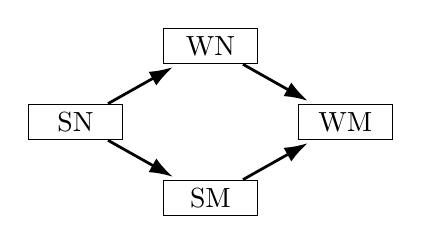
\begin{tikzpicture}[auto,
            arrowstyle/.style={->, line width=1pt, >={Latex[length=3mm, width=2mm]}, shorten >=2pt}]
            % A box style
            \tikzstyle{boxnode} = [draw, rectangle, text centered,minimum width=1.2cm, inner sep=3pt]   
            % Define the nodes
            \node (SN) [boxnode] at (4,0) {$\SN$};
            \node (WN) [boxnode, above right=0.5cm and 0.5cm of SN] {$\WN$};
            \node (SR) [boxnode, below right=0.5cm and 0.5cm of SN] {$\SM$};
            \node (WR) [boxnode, below right=0.5cm and 0.5cm of WN] {$\WM$};
            
            % Draw the arrows to form a diamond
            \draw [arrowstyle] (SN) -- (WN);
            \draw [arrowstyle] (SN) -- (SR);
            \draw [arrowstyle] (WN) -- (WR);
            \draw [arrowstyle] (SR) -- (WR);
        \end{tikzpicture}
        \caption{A hierarchy of normalizing and minimal properties.}
        \label{fig:norm-hierarchy}
\end{figure}

The implications will be explored in detail in Section \ref{sec:Implications}. 

A trivial implication not captured in the above figure is covered in Proposition \ref{prop:nftomf}. 
\begin{proposition}\label{prop:nftomf}
    $a\in NF_R \implies a \in MF_R$ 
\end{proposition}    
\begin{proof}
    See, \verb|NF ⊆ MF : ∀x → NFx → MFx| in \texttt{ARS-Implications.agda}.
\end{proof}

\begin{definition} The following definitions relate to confluence. Let $A$ and $R$ be as above, and let $a \in A$.
    \begin{description}
        \item[$a \in \WCR_R$] \emph{$a$ is weakly Church-Rosser (or weakly confluent)} if $c \bstep a \rstep b \implies c \mstep d \bmstep b$.
        \item[$a \in \CR_R$] \emph{$a$ is Church-Rosser (or confluent)} if $c \bmstep a \mstep b \implies c \mstep d \bmstep b$.
        \item[$a \in \NPe_R$] \emph{$a$ has the equivalence normal form property} if $a \estep b \implies a\mstep b$ for any $b \in \NF$.
        \item[$a \in \NP_R$] \emph{$a$ has the normal form property} if $c \bmstep a \mstep b \implies c \mstep b$ for any $b \in \NF$\footnote{In \terese $\NF$ is used to denote $\NPe$, whereas we have chosen to use $\NF$ to denote normal form.}. 
        \item[$a \in \MP_R$] \emph{$a$ has the minimal form property} if $c \bmstep a \mstep b \implies c \mstep b$ for any $b \in \MF$.
        \item[$a \in \UN_R$] \emph{$a$ has the unique normal form property} if $a \estep b \implies a \equiv b$  for any $a, b \in NF$.
        \item[$a \in \UNto_R$] \emph{$a$ has the unique normal form property with respect to reduction} if $c \bmstep a \mstep b  \implies b \equiv c$  for any $b, c \in NF$.
    \end{description}
\end{definition}

Again, we found that there was a strong interrelationship between the properties, captured in Figure \ref{fig:conf-hierarchy}, which are explored in Section \ref{sec:Implications}.

\begin{figure}[h] 
    \centering

        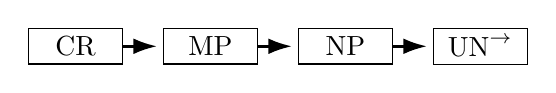
\begin{tikzpicture}[auto,
          arrowstyle/.style={->, line width=1pt, >={Latex[length=3mm, width=2mm]}, shorten >=2pt}]
          % A box style
          \tikzstyle{boxnode} = [draw, rectangle, text centered,minimum width=1.2cm, inner sep=3pt]
      
          % Place the nodes vertically (top to bottom)
          \node (Confluent) [boxnode] at (-4,0) {$\CR$};
          \node (RP)        [boxnode, right=.5cm of Confluent] {$\MP$};
          \node (WN)        [boxnode, right=.5cm of RP] {$\NP$};
          \node (UN)        [boxnode, right=.5cm of WN] {$\UNto$};
      
          % Draw arrows downwards
          \draw[arrowstyle] (Confluent) -- (RP);
          \draw[arrowstyle] (RP) -- (WN);
          \draw[arrowstyle] (WN) -- (UN);
       
          \end{tikzpicture}
          \caption{A hierarchy of confluent properties.}
          \label{fig:conf-hierarchy}
    
\end{figure}

\sacomment{Make sure somewhere it is mentioned that NP equals $NP_=$ and that UN does not equal UNto.}


\sacomment{Work for Saturday: Get the final definitions written up: namely the RP definitions and maybe make a figure to show those interrelationships}.
%     \begin{definition}
    
%   An element $a \in A$ is \emph{R-weakly confluent} ($WCR_R$) if all single step relations from $a$ can always converge
%     via multi-step relations to some common reduct.

%     A relation $R$ is \emph{weakly confluent} (AKA weakly Church-Rosser (WCR)) if every $a \in A$ is R-weakly confluent.
% \end{definition}

% \begin{definition}
%     An element $a \in A$ is \emph{R-confluent} ($CR_R$) if all multi-step relations from $a$ can always converge
%     via multi-step relations to some common reduct.
%     A relation $R$ is \emph{confluent} (AKA Church-Rosser (CR)) if every $a \in A$ is R-confluent.
% \end{definition}

\begin{definition}
  \label{d:WFacc}
  An element is \emph{accessible} if ...
\end{definition}

% \begin{definition}
%     An element $a \in A$ is \emph{$R$-weakly normalizing} ($WN_{R}$)if $a \mstep b$ for some normal form $b \in A$.

%     A relation $R$ is weakly normalizing (WN) if every $a \in A$ is $R$- weakly normalizing.
% \end{definition}

% \begin{definition}
%     An element $a \in A$ is \emph{$R$-strongly normalizing} ($SN_R$) if every sequence of relations starting from $a$ is finite.

%     A relation $R$ is strongly normalizing (SN) if every
%     $a \in A$ is $R$-strongly normalizing.
% \end{definition}

The above definition of SN is taken from [TeReSe].
When working in Agda, we make use of the alternative definition presented in [TeReSe] ($\leftarrow$ is accessibly well-founded).
The \ref{sec:Well-foundedness} section clarifies this definition.

% \begin{definition}
%     An element $a \in A$ has the \emph{$R$-weak normal form property} ($WNFP_{R}$) if $a \mstep b$ and
%     $a \mstep c \implies c \mstep b$, for all $c \in A$ and all normal form $b \in A$.

%     A relation $R$ has the \emph{weak normal form property} (WNFP) if every $a \in A$ has the $R$-weak normal form property.
% \end{definition}

% \begin{definition}
%     The \emph{equivalence relation} of $R$ is the smallest relation $\estep$ that contains $R$ and is reflexive, transitive, and symmetric.
% \end{definition}

% \begin{definition}
% An element $a \in A$ has the \emph{$R$-normal form property} ($NFP_{R}$) if
% $a \estep b$  $\implies$
% $a \mstep b$, for any normal form $b \in A$.

% A relation $R$ has the \emph{normal form property} (NFP) if every $a \in A$ has the $R$-normal form property.
% \end{definition}

% In ARS-Implications.agda we show the equivalence of WNFP and NFP when applied globally in the function $\mathtt{NP \leftrightarrow WNFP}$.

% In the next definition we deonte two elements $a, b \in A$ being equivalent with $a \equiv b$.
% \begin{definition}
% An element $a \in A$ has the \emph{{R}-unique normal form property} ($UN_{R}$) if
% $a \estep b$  $\implies$
% $a \equiv b$, for any normal form $b \in A$.

% A relation $R$ has the \emph{unique normal form property} ($UN$) if every $a \in A$ has the $R$-unique normal form property.
% \end{definition}


% \begin{definition}
% An element $a \in A$ has the \emph{${R}$-unique normal form property with respect to reduction} ($UN^ \to _{R}$) if
% $b \bmstep  \cdot  \mstep c$  $\implies$ $b \equiv c$, for all normal forms $b,c \in A$.

% A relation $R$ has the \emph{unique normal form property with respect to reduction} ($UN^\to$) if every $a \in A$ has the
% $R$-unique normal form property with respect to reduction.
% \end{definition}
% In ARS-Implications.agda we show that $UN$ implies $UN\to$ but the inverse implication doesn't hold, as seen
% in counterexample (\sacomment{TODO: put counterexample here when section is complete}).

\begin{definition}
    A \emph{sequence (in $A$)} is a function from the natural numbers to $A$:
    \begin{align*}
      &s : \nat \to A \\
      &s = (s_0,s_1,s_2,\dots)
    \end{align*}
\end{definition}

\begin{definition}
    A sequence is \emph{$R$-increasing} if every term is $R$-related to its preceding term.
\end{definition}

\begin{definition}
    A sequence is \emph{bounded} if there exists an element $a \in A$ to which all elements of the sequence reduce.
\end{definition}


% \begin{definition}
%     An element $a \in A$ has the \emph{minimal form property} ($MF$) if $a \mstep b \implies b \mstep a$ for all $b \in A$.
% \end{definition}

% Note that being a normal form is a trivial case of the minimal form property (as we prove in ARS-implications.agda
% function $\mathtt{NF\subseteq MF : \forall {x} \to NF x \to MF x}$).

\begin{definition}\label{d:RP}
    A relation $R$ has the \emph{recurrence property} (RP) if every bounded, increasing sequence 
    has an element $a \in MF$.
\end{definition}


\begin{definition}\label{d:RP-}
    A relation $R$ has the \emph{weak recurrence property} (RP-) if for every increasing 
    sequence with bound $a$, there is an element $i$ of the sequence such that 
    $a \mstep f(i)$.
\end{definition}


% \begin{definition}
%     An element $a \in A$ is \emph{$R$-weakly minimal} ($WM_{R}$)if $a \mstep b$ for some minimal form $b \in A$.

%     A relation $R$ is weakly minimal (WM) if every $a \in A$ is $R$-weakly minimal.
% \end{definition}

% \begin{definition}
%     An element $a \in A$ is \emph{$R$-strongly minimal} ($SM_R$) if either $a$ itself is a minimal form or every element one $R$ step
%     from $a$ is also strongly minimal.

%     A relation $R$ is strongly minimal (SM) if every
%     $a \in A$ is $R$-strongly minimal.
% \end{definition}

% \begin{definition}
%    An element $a \in A$ has the \emph{${R}$-weak minimal form property} ($WMFP_R$) if
%    $a \mstep b$ and $a \mstep c$  $\implies$
%    $c \mstep b$, for all $c \in A$ and all $b \in A$ with the minimal form property.

%    A relation $R$ has the \emph{weak minimal form property} (WMFP) if every $a \in A$ has the $R$-weak minimal form property.
% \end{definition}
\begin{definition}
    \label{d:inc}
    A relation $R \sse A \times A$ is called \emph{increasing} if there
    exists a ``size function'' $|-| : A \to \nat$ satisfying, for all $x, y \in A$,
    \[ Rxy \to |x| < |y| \]
\end{definition}

Definitions to add:
\begin{enumerate}
    \item Finite branching
    \item Any other terms from well foundedness
    \item The other terms we have for strongly
\end{enumerate}

\section{Formalization of \terese}
\label{sec:Formalization}
This sections is a guide to our formalization of \terese $\,$ and explains the deviations we take from the text.

\subsection{Formalization of Definitions (\texttt{Base.agda})}\label{subsec:def}

As outlined in the previous section, \texttt{Properties.agda}, \texttt{Seq.agda}, and \texttt{ClosureOperators.agda} define most standard termination and confluence properties. The file \texttt{Base.agda} introduces additional definitions which are required for the formalization of the propositions found in Chapter 1 of \terese.


The following is a summary of the differences in definitions we have used as mentioned in Section \ref{sec:Definitions}.
\begin{itemize}
    \item $\SN$ : We define this via the notion of accessibility rather than the non-existence of infinite reduction sequences. Both definitions articulate normalization as well-foundedness of the converse relation. However, different notions of well-foundedness are used in the two definitions. The differences are highlighted in Section~\ref{sec:Well-foundedness}.
     See Section \ref{sec:Well-foundedness} for further discussion.
    \item $\NPe$ : We use the equivalent $\NP$ definition.
    \item $\Inc$ : We use the more general property $\RP$.
\end{itemize}

As mentioned, the $\Inc$ property can impose a computationally demanding requirement. However, $\Inc$ is used only in Theorem 1.2.3
and the only crucial aspect of $\Inc$ needed for the proof is that no $R$-increasing
sequence can have an upper bound.
We establish that the weaker property $\RP$ (or its equivalent $\RPm$) is sufficient for replacing $\Inc$ in the theorem (see Subsection \ref{subsec:theorems}).
This led us to examine the condition on $s (i)$ appearing inside $\RP$ more closely. This condition provides a generalization of the notion of a normal form,
which we explore in detail in Section \ref{sec:Hierarchy}.

\subsection{\texttt{Propositions.agda}}
There are three sets of propositions given in \terese: \texttt{1.1.9}, \texttt{1.1.10}, \texttt{1.1.11}.
The formalization of the proofs are in \texttt{Propositions.agda}. These formalizations are straightforward
and do not merit further discussion.

\subsection{\texttt{Theorems.agda}} \label{subsec:theorems}

\begin{theorem}(Newman's Lemma)
  $\gSN \land \gWCR \implies \gCR$
\end{theorem}

\begin{proof}
  There are three proofs of Newman's Lemma given in \terese.
  The first and third of these proofs make use of classical reasoning. The second proof is amenable to a
  constructive formalization as shown in the following function in \texttt{ARS-NewmansLemma.agda}:

  \verb|NewmansLemma : R isSN → R isWCR → R isCR|.
\end{proof}

  We show in Subsection \ref{subsec:newnewman} a generalization of Newman's Lemma using a condition distilled from $\gRP$.
  The formalizations of the remaining theorems are all found in \texttt{Theorems.agda}.

\begin{theorem}[Thm 1.2.2 in \terese]
\begin{enumerate}[label=\roman*.]
  \item[]
  \item $\gCR \implies \gNPe \implies \gUN$
  \item $\gWN \land \gUN \implies \gCR$
  \item $\gCRs \implies \gCR$
\end{enumerate}
\end{theorem}

\begin{proof}
    See \texttt{module Theorem-1-2-2} in \texttt{Theorems.agda}, \\
    \verb|CR→NP : R isCR → R isNP₌|\\
    \verb|NP→UN : R isNP₌ → R isUN|\\
    \verb|ii     : R isWN × R isUN → R isCR|\\
    \verb|ii+    : R isWN × R |\texttt{isUN}$^{\to}$ \verb|→ R isCR|\\
    \verb|iii    : subcommutative R → R isCR|
\end{proof}
\begin{remark}
    In $\mathtt{UN^{→}∧WN→CR}$ a more general proof of ($ii$) is given using $\UNto$.
\end{remark}


\begin{theorem}[Thm. 1.2.3 in \terese]
  \begin{enumerate}[label=\roman*.]
    \item[]
    \item $\gWN \land \gUN \implies \gBP$
    \item $\gBP \land \gInc \implies \gSN$
    \item $\gWCR \land \gWN \land \gInc \implies \gSN$
    \item $\gCR \iff \gCP$ $($the forward implication only holds if the ARS is countable.$)$
  \end{enumerate}
\end{theorem}

\begin{proof}
    See \texttt{module Theorem-1-2-3} in \texttt{Theorems.agda},\\
    \verb|i     : R isWN → R isUN → R isBP|\\
    $\mathtt{i^\to}$\hspace{5mm} \verb|: R isWN → R |\texttt{isUN}$^{\to}$ \verb|→ R isBP|\\
    \verb|iiSeq : R isWN → R isUN → R isRP → isWFseq- (~R R)|\\
    \verb|iii   : R isWN → R isWCR → R isRP- → dec SN → R isSN|\\
    \verb|iv    : R isCP → R isCR|
\end{proof}
\begin{remark} \hfill
  \begin{description}
    \item[($i$)] In $\mathtt{i^\to}$ we again provide a slight improvement by using $\gUNto$ rather than $\gUN$.
    \item[($ii$)] This proof is inherently classical. For the closest constructive analogue to this proof we have written $\mathtt{iiSeq}$, where we replace $\gBP$ with the stronger properties $\gWN$ and $\gUN$ and we replace $\gInc$ with the weaker property $\gRP$.
    With the original property $\gBP$ and $gRP$ we can imply the related property $gSM$ ($\gSM$ is defined in Section~\ref{sec:Hierarchy} and its relation to $gSN$ is expanded upon). The definition and further discussion of $\isWFseqm$ are provided in Section~\ref{sec:Well-foundedness}.
    \item[($iii$)] In $\mathtt{iii}$, we replace $\gInc$ with the more general property $\gRPm$. We also assume that $\gSN$ is decidable, as this allows the construction of a witness for whether an element possesses the property $\SN$, which is essential for our proof.
  \end{description}
\end{remark}

\section{Implications}
\label{sec:Implications}

From the perspective of programming language theory, the two properties of abstract rewriting 
systems that are most interesting are $\SN$ and $\CR$. The following hierarchies 
show chains of implications starting from these properties.

\begin{center}

    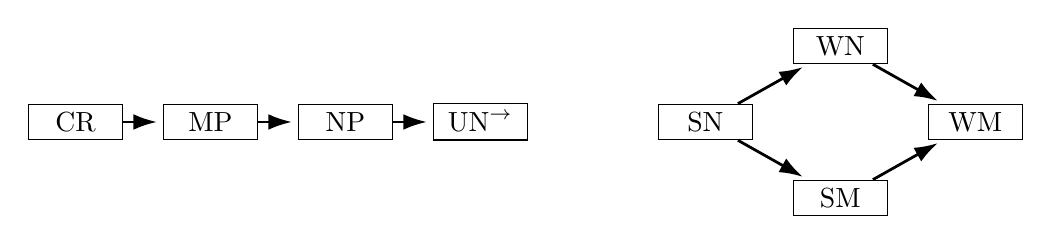
\begin{tikzpicture}[auto,
      arrowstyle/.style={->, line width=1pt, >={Latex[length=3mm, width=2mm]}, shorten >=2pt}]
      % A box style
      \tikzstyle{boxnode} = [draw, rectangle, text centered,minimum width=1.2cm, inner sep=3pt]
  
      % Place the nodes vertically (top to bottom)
      \node (Confluent) [boxnode] at (-4,0) {$\CR$};
      \node (RP)        [boxnode, right=.5cm of Confluent] {$\MP$};
      \node (WN)        [boxnode, right=.5cm of RP] {$\NP$};
      \node (UN)        [boxnode, right=.5cm of WN] {$\UNto$};
  
      % Draw arrows downwards
      \draw[arrowstyle] (Confluent) -- (RP);
      \draw[arrowstyle] (RP) -- (WN);
      \draw[arrowstyle] (WN) -- (UN);
   
        
        % Define the nodes
        \node (SN) [boxnode] at (4,0) {$\SN$};
        \node (WN) [boxnode, above right=0.5cm and 0.5cm of SN] {$\WN$};
        \node (SR) [boxnode, below right=0.5cm and 0.5cm of SN] {$\SM$};
        \node (WR) [boxnode, below right=0.5cm and 0.5cm of WN] {$\WM$};
        
        % Draw the arrows to form a diamond
        \draw [arrowstyle] (SN) -- (WN);
        \draw [arrowstyle] (SN) -- (SR);
        \draw [arrowstyle] (WN) -- (WR);
        \draw [arrowstyle] (SR) -- (WR);
      \end{tikzpicture}
\end{center}
  
The classical property of being minimally decidable is required to complete the implcation 
from $\SN$ to $\WN$, as can be seen in our formalization

\verb|SNdec→WN : (~R R) isMinDec → SN ⊆ WN| \footnotemark[1]

\sacomment{Are we going to define this property here or elsewhere?}

The isMinDec property states that all elements either have a relation to some other element, or 
there is no other element to which they have a relation. If the element relates to no other element then it is terminating 
and so trivially $\WN$. If the element does relate to some other element $y \in A$, then we recursively apply our claim to 
$y$ and because we know that we have the property of $\SN$ we must eventually reach a terminating element. 

Similarly, the property of being minimally decidable is required in order to show that $\SM$ implies $\WM$.

The following tables show which combination of these properties implies a property higher in the hierarchy. Where a combination 
does not imply a higher property an explanatory counterexample is given. The counterexamples referenced are in section \ref{sec:Counterexamples}.

The first table explores where the properties hold locally, the second explores where the properties hold globally. The proofs that the 
following implications hold are primarily found in \texttt{ARS-implications.agda} unless they have been proven as part of the formalization 
of \terese, in which case they will be found in either \texttt{ARS-thoerems.agda} or \texttt{ARS-NewmansLemma.agda}.


\sacomment{UPDATE COUNTEREXAMPLES WHEN CE SECTION FINISHED}
\renewcommand*{\thefootnote}{\fnsymbol{footnote}}
\begin{table}[h!]
    \centering
    \caption{Local implications}
    \begin{tabular}{|>{\columncolor{gray!30}}l|c|c|c|c|c|}
    \hline
    \rowcolor{gray!30}     & $\WM$         & $\WN$         & $\SM$             & $\SMandWN$        & $\SN$ \\
    \hline
    $\UNto$ &  CE-, CE-     & CE, CE-       & $\CR$\footnotemark[1] , CE-          & $\CR$\footnotemark[1], CE            & $\CR$\footnotemark[2] , $\SN$ \\
    \hline
    $\NP$ & CE-, CE-      & $\CR$, CE-    & $\CR$\footnotemark[1] , CE-          & $\CR$, $\SN$      & $\CR$\footnotemark[2] , $\SN$ \\
    \hline
    $\MP$ & $\CR$ , CE-    & $\CR$, CE-    & $\CR$\footnotemark[2] , CE- & $\CR$, $\SN$      & $\CR$\footnotemark[2] , $\SN$ \\
    \hline
    $\CR$   & $\CR$, CE-     & $\CR$, CE-     & $\CR$, CE-        & $\CR$, $\SN$     & $\CR$ , $\SN$ \\
    \hline
    
    \end{tabular}
\end{table}
\begin{table}[h!]
    \centering
    \caption{Global implications}
    \begin{tabular}{|>{\columncolor{gray!30}}l|c|c|c|c|c|}
    \hline
    \rowcolor{gray!30}     & $\WM$         & $\WN$         & $\SM$             & $\SMandWN$        & $\SN$ \\
    \hline
    $\UNto$ &  CE-, CE-     & $\CR$, CE-    & $\CR$\footnotemark[1] , CE-          & $\CR$, $\SN$      & $\CR$\footnotemark[2] , $\SN$ \\
    \hline
    $\NP$ & CE-, CE-      & $\CR$, CE-    & $\CR$\footnotemark[1] , CE-          & $\CR$, $\SN$      & $\CR$\footnotemark[2] , $\SN$ \\
    \hline
    $\MP$ & $\CR$ , CE    & $\CR$, CE-    & $\CR$\footnotemark[2] , CE- & $\CR$, $\SN$      & $\CR$\footnotemark[2] , $\SN$ \\
    \hline
    $\CR$   & $\CR$, CE     & $\CR$, CE     & $\CR$, CE-        & $\CR$, $\SN$      & $\CR$ , $\SN$ \\
    \hline
    
    \end{tabular}
\end{table}
\footnotetext[1]{This implication also requires global $\WCR$.}
\footnotetext[2]{This implication also requires either global $\WCR$ or the classical property required to go from 
$\SN \to \WN$ or $\SM \to \WM$.}
\renewcommand*{\thefootnote}{\arabic{footnote}}


\sacomment{Need to update the tables with appropriate symbols for global and local. Colour for first row and column?}

The tables show that there are two changes when moving from properties holding locally to globally. 
Globally $\WN \land \UNto \implies \CR$ holds whereas it does not locally. Similarly, $\SM \land \WN \implies \SN$ holds 
globally but not locally. 

Theorem 1.2.2 ii in \terese is the claim that $\WN \land \UN \implies \CR$ holds, and we formalize this in

\verb|ii : R isWN × R isUN → R isCR| \footnotemark[3]

We have modestly generalized this theorem by showing that $\WN \land \UNto \implies \CR$ holds (and indeed this is the basis for our proof of the theorem). 
Counterexample \sacomment{REF HERE} shows why this implication cannot hold when the properties are only local. Our proof is in the function:

\verb|UN→∧WN→CR : R isUN→ → R isWN → R isCR| \footnotemark[1]

To show that $\SM \land \WN \implies \SN$ we built on our proof that locally $\SM \land \WN \land \NP \implies \SN$. If $\WN$ applies 
globally then our proof no longer requires the property $\NP$. This progression of proofs can be seen in the functions:

\verb|WN∧NP∧SM→SN : ∀ {x} → WN x → NP x → SM x → SN x| 

\verb|isWN∧SM→SN : R isWN → ∀ {x} → SM x → SN x|

\verb|isWN∧isSM→isSN : R isWN → R isSM → R isSN| \footnotemark[1]
\section{Well-foundedness}

\newcommand{\then}{\Longrightarrow}
\label{sec:Well-foundedness}

% \newcommand{\accCor}{\textbf{accCor}}
% \newcommand{\accDNE}{\textbf{accDNE}}

% We use Well-founded not Wellfounded

\newcommand{\gWF}{\mathbf{WF}}
\newcommand{\WF}{\mathrm{WF}}

An abstract reduction $\to_R$ is strongly normalizing
if and only if the converse relation is well-founded.
In this section, we will compare several definitions of well-foundedness.
For ease of exposition, we will only consider local versions of these notions.
(There is no loss of generality in this; any global well-foundedness property $\gWF(A;R)$ 
restricts to a predicate $WF_R$ on $A$ via $WF_R(x) = \gWF(\Sigma y : A. R^* x y;R')$, 
where $R'((y,\rho),(z,\sigma)) = R(y,z)$.)
%which depend on the basic notions given in Definition~\ref{def:WFnotions} below.

\subsection{Definitions of well-foundedness}

For the rest of this section, fix $R \subseteq A \times A$.  We write $Rxy$ for $(x,y) \in R$.

In the context of ARS, the reader should think of the converse relation,
interpreting $Rxy$ as denoting a reduction step $y \to_R x$.

For $P \subseteq A$, let $\ol{P} = \{ x \in A \mid x \notin P\}$ denote the complement of $P$.
\begin{definition}\label{def:WFnotions} \hfill
   \begin{enumerate}
    \item $x \in A$ is \emph{accessible} if for all $y \in A$, $Ryx$ implies $y$ is accessible.
      This is an inductive definition, with the base case obtained at
     those $x$ satisfying $\lnot Ryx$ for all $y$.
    \item $P \subseteq A$ is \emph{inductive}
    if, for each $x \in A$, $(\forall y. Ryx \to y \in P)$ implies $x \in P$.


    \item $x \in A$ is \emph{$P$-minimal} if $x \in P$ and for all $y$,
    $Ryx$ implies $y \notin P$.

    \item $P \subseteq A$ is \emph{coreductive} if, for each $x \in \ol{P}$, there is a $y \in A$ such that $Ryx$ and $y \in \ol{P}$.

    % \item $s : \nat \to A$ is \emph{$R$-decreasing} if for all $k$, $(s(k+1),s(k)) \in R$.
  \end{enumerate}
\end{definition}

The above notions give rise to several distinct definitions of well-foundedness, given below.
Recall the definition of an $R$-decreasing sequence from Section~\ref{sec:Definitions}:
this is a function $s : \nat \to A$ satisfying $R(s(k+1))(sk) \in R$ for all $k \in \nat$.

\begin{definition} \label{def:WFproperties} \hfill
  \begin{enumerate}
    \item $R$ is \emph{accessibly well-founded} ($\WFacc$) if every element is accessible:
      \[
        \forall x \in A.\; x \text{ is accessible}
      \]
    \item \label{def:WFind} $R$ is \emph{inductively well-founded} ($\WFind$) if every inductive predicate is universally true:
      \[
        \forall P \subseteq A.\;\text{$P$ is inductive} \Rightarrow \forall x \in A.\; x \in P
      \]
    \item $R$ is \emph{coreductively well-founded} ($\WFcor$) if every coreductive predicate is universally true:
      \[
        \forall P \subseteq A.\;\text{$P$ is coreductive} \Rightarrow \forall x \in A.\; x \in P
      \]
    \item  $R$ is \emph{well-founded minimality-wise} ($\WFmin$) if every nonempty subset contains a minimal element:
      \[
        \forall P \subseteq A.\; P \neq \varnothing \Rightarrow
        \exists x \in A.\; \text{$x$ is $P$-minimal}
      \]
    \item  $R$ is \emph{well-founded minimality-wise for $\lnot \lnot$-closed predicates} ($\WFminDNE$) if every nonempty $\lnot \lnot$-closed subset contains a minimal element:
      \[
        \forall P \subseteq A.\; P \neq \varnothing \Rightarrow \ol{\ol P} \subseteq P \Rightarrow
        \exists x \in A.\; \text{$x$ is $P$-minimal}
      \]
   \item $R$ is \emph{sequentially well-founded} ($\WFseq$) if every sequence contains an index at which it is not decreasing:
      \[
        \forall s : \nat \to A\ \exists k : \nat.\, \lnot \, R \,(s\,(k+1))\,(s\,k)
      \]
  \end{enumerate}
\end{definition}
We have formalized the above definitions of well-foundedness in \texttt{WFDefinitions.agda}.

Classically, the above notions of well-foundedness are all equivalent.  Constructively, only the first two are equivalent; the remaining definitions are not. Moreover, even individual classical definitions can be given constructive
interpretations in varying degrees of logical strength.
Formalizing the remaining implications enabled us to identify where exactly classical logic
is used, and how much of it is truly needed.

For example, the implication from ``every non-empty subset has a minimal element'' to
``every element is accessible''  is a classical proof by contradiction.
(Assuming that there exists an inaccessible element, the hypothesis implies that
there must be a minimal such element, which immediately yields a contradiction:
every minimal element is accessible.)

Constructively, this argument only goes so far as to show that, if every non-empty
subset has a minimal element, then no element is inaccessible.
That is, the universal statement being proved is that every $x \in A$
is not-not-accessible. The final step needed to infer that $x$ is indeed accessible
is not constructively provable in general, therefore it needs to be assumed as
an additional hypothesis in order to recover the full implication.

On the other hand, assuming accessibility is $\lnot\lnot$-closed, the other
hypothesis can now be weakened, to only require existence of minimal elements
for $\lnot\lnot$-closed subsets.  This is a significant restriction, which may
be validated in certain cases.  In contrast, the original hypothesis
(postulating minimal elements for ALL predicates)
is generally equivalent to every subset being decidable.
The file \texttt{WFCounters.agda} shows that assuming the full minimality hypothesis $\WFmin$ for the standard strict order on the natural numbers entails decidability of every subset of $\nat$ (which is clearly incompatible with effective semantics), while its restriction $\WFminDNE$ implies
%(and is equivalent to)
that each subset $P$ is \emph{weakly} decidable,
satisfying $\lnot \lnot P(x) \lor \lnot P(X)$ for all $x$.

One could also consider proving well-foundedness ``up to $\lnot\lnot$'',
asserting that every element is $\lnot\lnot$-accessible,
every sequence $\lnot\lnot$-contains a non-decreasing index,
for every non-empty subset there $\lnot\lnot$-exists a minimal element, etc.
These weaker notions are formalized in the definition below, and in the corresponding file
\texttt{WFWeakDefinitions.agda}.

\begin{definition} \label{def:WFweakproperties} \hfill
  \begin{enumerate}
    \item $R$ is \emph{weakly accessibly well-founded} ($\WFaccm$) if accessibility holds for all elements up to double negation:
      \[
        \forall x \in A.\; \lnot \lnot  (x \text{ is accessible})
      \]
    \item $R$ is \emph{weakly inductively well-founded} ($\WFindm$) if every inductive predicate holds for all elements up to double negation:
      \[
        \forall P \subseteq A.\;\text{$P$ is inductive} \Rightarrow \forall x \in A.\; \lnot \lnot (x \in P)
      \]
    \item $R$ is \emph{weakly coreductively well-founded} ($\WFcorm$) if every coreductive predicate holds for all elements up to double negation:
      \[
        \forall P \subseteq A.\;\text{$P$ is coreductive} \Rightarrow \forall x \in A.\; \lnot\lnot(x \in P)
      \]
    \item  $R$ is \emph{weakly well-founded minimality-wise} ($\WFminm$)
      if for every nonempty subset $P$ there $\lnot \lnot$-exists a minimal element in $P$:
      \[
        \forall P \subseteq A.\; P \neq \varnothing \Rightarrow \lnot \lnot \;
        (\exists x \in A.\; \text{$x$ is $P$-minimal})
      \]
    \item  $R$ is \emph{weakly well-founded minimality-wise for $\lnot \lnot$-closed predicates} ($\WFminDNEm$)
      if for every nonempty $\lnot \lnot$-closed subset $P$ there $\lnot \lnot$-exists a minimal element in $P$:
      % \[
      %   \forall P \subseteq A.\; P \neq \varnothing \Rightarrow \left(\ol{\ol P} \subseteq P\right) \Rightarrow \lnot \lnot \;
      % (\exists x \in P.\; \text{$x$ is $P$-minimal}) \]
      \[
        \forall P \subseteq A.\; P \neq \varnothing \Rightarrow \ol{\ol P} \subseteq P\Rightarrow \lnot \lnot \;
        (\exists x \in A.\; \text{$x$ is $P$-minimal})
      \]
  \item $R$ is \emph{weakly sequentially well-founded} ($\WFseqm$) if no sequence is $R$-decreasing:
    \[
      \forall s:\nat \to A.\; \lnot \text{($s$ is $R$-decreasing)}
    \]
\end{enumerate}
\end{definition}

In \terese, the $\WFseqm$ definition is used, as in the classical mathematics textbooks. Constructively, this is not a useful definition, as it does not provide any positive computational content and requires an explicit sequence to be defined.  This definition appears to be strictly weaker than
$\WFseqnn$, asserting that every sequence not-not contains a
non-decreasing index.

% \apcomment{Perhaps we should have a separate discussion between isWFseq- and isWFseq-not-not?}

\subsection{Implications between the definitions}

The logical relationships between all of the above definitions are summarized in Figure~\ref{fig:WF}.
All of the implications in the figure have been
formalized within the WellFounded subdirectory of the Agda repository.
An arrow from one node to another with no label indicates direct logical implication,
provable constructively with no additional assumptions. An arrow with a label indicates an additional
(semi-)classical hypothesis needed to establish the implication.
The definitions of these hypotheses are given in Figure \ref{tab:cprop}.

We consider $\WFacc$ to be the canonical constructive definition of
a well-founded relation (hence the emphasis in the figure).
In the ARS setting, this corresponds to defining
strong normalization inductively in terms of reductions to normal forms.
As can be seen from the figure, it is implied by
Terese's definition $\WFseqm$ only when \emph{two}
strongly classical conditions are in place.
These are $\accDNE$ (not-not-closure of strong normalization)
and $\accCor$ (which is related to the existence of an effective perpetual reduction strategy).

% \begin{figure}[h]
% \centering
% \begin{tikzpicture}[
%   scale=0.7,
%   every node/.style={transform shape},
%   node distance=1cm and .5cm,
%   box/.style={draw, rectangle, rounded corners, minimum width=1cm, minimum height=1cm, align=center},
%   arrow/.style={-{Latex}, thick}
% ]

% % Row 1: WFmin -> WFmin-
% \node[box] (WFmin) {$\WFmin$};
% \node[box, right=2.9cm of WFmin] (WFminM) {$\WFminm$};

% \draw[arrow] (WFmin) -- (WFminM);

% % Row 2: WFminDNE -> WFminDNE-
% \node[box, below=of WFmin] (WFminDNE) {$\WFminDNE$};
% \node[box, below=of WFminM] (WFminDNEM) {$\WFminDNEm$};

% \draw[arrow] (WFminDNE) -- (WFminDNEM);

% % Row 3: WFacc

% \node[box, line width = 0.5mm, below=of WFminDNE] (WFacc) {$\WFacc$};

% \node[box, below = of WFminDNEM] (WFaccM) {$\WFaccm$};
% \draw[arrow] (WFacc) to (WFaccM);
% \draw[arrow, bend left] (WFaccM) to node[below, text=red] {$\accDNE$} (WFacc);


% % Row 4: WFseq
% \node[box, below=of WFacc] (WFseq) {$\WFseq$};
% \node[box, below= of WFaccM] (WFseqM) {$\WFseqm$};

% \draw[arrow] (WFseq) -- (WFseqM);

% % Row 5: WFcor
% \node[box, below=of WFseq] (WFCor) {$\WFcor$};
% \node[box, below=of WFseqM] (WFminCor) {$\WFcorm$};

% % \draw[arrow, bend left = 55] (WFaccM) to (WFminM);

% % Inter-row arrows
% \draw[arrow] (WFacc) to node[right, text = red] {$\rdec$} (WFseq);
% \draw[arrow, bend right] (WFaccM) to (WFminDNEM);
% \draw[arrow, bend right = 90] (WFminCor) to node[pos = 0.4, right, text=red] {$\accCor$} (WFaccM);

% \draw[arrow, bend right = 75] (WFmin) to (WFseq);
% \draw[arrow, bend left = 75] (WFminM) to (WFseqM);
% \draw[arrow] (WFaccM) -- (WFseqM);
% \draw[arrow] (WFmin) -- (WFminDNE);
% \draw[arrow, bend right] (WFminM) to (WFminDNEM);
% \draw[arrow, bend right] (WFminDNEM) to (WFminM);

% \draw[arrow] (WFminDNE) to node[right, text = red] {$\accDNE$} (WFacc);
% \draw[arrow, bend right=45] (WFminDNE) to node[pos=0.3, left, text=red] {$\mpe$} (WFseq);
% \draw[arrow, bend right] (WFminDNEM) to node[left, text=red] {$\FB$} (WFaccM);
% \draw[arrow, bend right] (WFseqM) to (WFminCor);
% \draw[arrow, bend right] (WFminCor) to node [right, text=red] {$\mpe$} (WFseqM);
% \draw[arrow] (WFCor) -- (WFminCor);
% % \draw[arrow, bend left = 110] (WFCor) to node[left, text=red] {$\accCor$} (WFacc);
% \draw[arrow, bend left] (WFminCor) to node[below, text=red] {$\corDNE$} (WFCor);

% \draw[arrow, bend left=80] (WFCor) to node[pos = 0.4, left, text=red] {$\accCor$} (WFacc);

% \end{tikzpicture}
% \caption{The logical relationships between notions of well-foundedness}
%  \label{fig:WF}
% \end{figure}
% % \clearpage

\begin{figure}[h]
\centering
\begin{tikzpicture}[
  scale=0.6,
  every node/.style={transform shape},
  node distance=1cm and .5cm,
  box/.style={draw, rectangle, rounded corners, minimum width=1cm, minimum height=1cm, align=center},
  arrow/.style={-{Latex}, thick}
]

% Row 1: Basic definitions
\node[box] (WFmin) {$\WFmin$};
\node[box, right=2.9cm of WFmin] (WFminDNE) {$\WFminDNE$};
\node[box, right=2.9cm of WFminDNE, line width = 0.5mm] (WFacc) {$\WFacc$};
\node[box, right=2.9cm of WFacc] (WFseq) {$\WFseq$};
\node[box, right=2.9cm of WFseq] (WFCor) {$\WFcor$};

% Row 2: Weak definitions
\node[box, below=2cm of WFmin] (WFminM) {$\WFminm$};
\node[box, below=2cm of WFminDNE] (WFminDNEM) {$\WFminDNEm$};
\node[box, below=2cm of WFacc] (WFaccM) {$\WFaccm$};
\node[box, below=2cm of WFseq] (WFseqM) {$\WFseqm$};
\node[box, below=2cm of WFCor] (WFminCor) {$\WFcorm$};

% Arrows within rows
\draw[arrow] (WFmin) -- (WFminDNE);
\draw[arrow, bend left=25] (WFmin) to (WFseq);

\draw[arrow] (WFminM) -- (WFminDNEM);
\draw[arrow] (WFaccM) -- (WFseqM);
\draw[arrow, bend right=35] (WFaccM) to (WFminDNEM);
\draw[arrow, bend right=35] (WFminDNEM) to (WFminM);
\draw[arrow, bend right=25] (WFminDNEM) to (WFseqM);
\draw[arrow] (WFseqM) -- (WFminCor);

% Inter-row arrows
\draw[arrow] (WFmin) -- (WFminM);
\draw[arrow] (WFminDNE) -- (WFminDNEM);
\draw[arrow] (WFacc) -- (WFaccM);
\draw[arrow] (WFseq) -- (WFseqM);
\draw[arrow] (WFCor) -- (WFminCor);

% Additional labeled arrows
\draw[arrow] (WFminDNEM) to node[above, text=red] {$\FB$} (WFaccM);
\draw[arrow, bend right=35] (WFminCor) to node[above, text=red] {$\mpe$} (WFseqM);
\draw[arrow, bend right=25] (WFCor) to node[above, text=red] {$\accCor$} (WFacc);
\draw[arrow] (WFminDNE) to node[below, text=red]{$\accDNE$} (WFacc);
\draw[arrow, bend left = 25] (WFminDNE) to node[below, text=red]{$\mpe$} (WFseq);
\draw[arrow, bend right = 45] (WFminCor) to node[right, text=red]{$\corDNE$} (WFCor);
\draw[arrow, bend right = 45] (WFaccM) to node[right, text=red]{$\accDNE$} (WFacc);
\draw[arrow] (WFacc) to node[below, text=red]{$\rdec$} (WFseq);
\draw[arrow, bend left=25] (WFminCor) to node[below, text=red]{$\accCor$} (WFaccM);

\end{tikzpicture}
\caption{The logical relationships between notions of well-foundedness}
\label{fig:WF}
\end{figure}


% All of the above definitions of well-foundedness are classically equivalent.
% But constructively, the only provable equivalence is between the inductive and accessible
% formluations, reflecting the fact that accessibility is defined as the least inductive predicate.
% Formalizing the remaining implications enabled us to identify where exactly classical logic
% is used, and how much of it is truly needed.

{
\def\arraystretch{1.3}
\begin{figure}[h!]
\small
\begin{tabular}{@{}l l l @{}}
\toprule
\textbf{Property} & \textbf{Definition}  &\textbf{Agda Code}  \\
\midrule
$\rdec$   & $R$ is decidable
          & $\forall$ \verb|{x} {y}| $\to$ \verb|EM (R x y)|\\
$\FB$     & $R$ is finitely branching
          & $\mathtt{\forall (a : A) \to \Sigma [ xs \in List A ] (\forall b \to R a b \to b \in{}List\, xs)}$ \\
$\mpe$    & Sequences are $\lnot\lnot$-closed
          & $\forall\ \mathtt{(f : \nat \to A) \to \lnot\lnot Closed
          (\lambda x \to \Sigma [ k \in \nat ] (f\, k \equiv x))}$ \\
$\corDNE$ & Coreductives are $\lnot\lnot$-closed
          & $\mathtt{\forall (P : \mathcal{P} A) \to R}$-$\mathtt{coreductive\ P \to \lnot\lnot Closed\ P}$\\
$\accDNE$ & Accessibility is $\lnot\lnot$-closed
          & $\lnot\lnot$\verb|Closed (R -accessible)| \\
$\accCor$ & Accessibility is coreductive
          & \verb|R -coreductive (R -accessible)| \\
\bottomrule
\end{tabular}
\centering
\caption{Classical Properties Used in the Well-Foundedness Diagram}
\label{tab:cprop}
\end{figure}
}
% \clearpage
% The principles appearing in the labels of Figure \ref{fig:WF} are valid for many rewriting systems,
% and are classically true.
Figure \ref{fig:WF} illustrates that the network of logical relationships between
constructive notions of well-foundedness is quite rich indeed.
Taking the $\lnot\lnot$-closures of
these notions cuts down some, but not all, of the complexity.
For example, the two minimality principles become equivalent.
% The implication from the inductive to sequential definition no longer requires
% decidability of $R$.
% On the other hand, the reverse
At the same time, the weak version of the sequential definition is unable to imply
the (weak) accessible one without an additional hypothesis $\accCor$,
which may be described as the constructive contrapositive of the definition of accessibility.
In the context of rewriting systems,
this condition asserts the existence of a function which maps any
element that is \emph{not} strongly normalizing to a one-step reduct of it having the same property.
Assuming $\accCor$, all notions of well-foundedness
are constructively equivalent up to $\lnot\lnot$.

Other observations that can be gleaned from the figure include the following.
\begin{enumerate}
  \item The implication from $\WFacc$ to $\WFseq$ requires the underlying relation to be decidable.
    This assumption is no longer necessary on the $\lnot\lnot$-translated side.
  \item $\WFmin$ is a very strong assumption and implies $\WFseq$ unconditionally.
  The more reasonable $\WFminDNE$ requires the image of every sequence to be $\lnot\lnot$-closed
  to complete the implication.  This condition can be considered as a special case of Markov's Principle
  (if one assumes that equality on $A$ is decidable).
  \item On the $\lnot\lnot$-side, $\WFminm$ and $\WFminDNEm$ are equivalent. Both are directly implied by $\WFaccm$,
    and all three directly imply $\WFseqm$.
  \item All definitions imply $\WFcorm$.  This weakest definition implies $\WFaccm$ assuming the
    ``constructive contrapositive of accessibility'', $\accCor$.
    %While this condition is implied by $\isWFseqm$, it does not appear to imply anything on its own.

    With this assumption, $\WFacc$ can also be derived from $\WFcor$. % , the stronger version of $\WFcorm$.

    % \apcomment{Remove?} (This is analogous to how $\isWFminDNE$ is a natural weakening of
    % $\isWFmin$ that is sufficient to recover $\isWFacc$ in the presence of {$\accDNE$}.)

  \item If the relation is finitely branching ($\FB$), then $\WFminDNEm$
    implies $\WFaccm$ directly.

    (It may be noted that $\FB$ implies $\accCor$ whenever the relation $R$ is decidable
    and $R$-accessibility is \emph{weakly} decidable;  this is proved in \texttt{Coreductive.agda}.)
  % \apcomment{The previous observation suggests the question of whether isWFseq- might
  % imply isWFminDNE- via decidability of minimal elements.\\
  % However, in trying to prove this implication, the hypothesis asserting non-existence of
  %  a minimal element of some given non-empty $\lnot\lnot$-closed predicate
  %  automatically entails that any particular element of interest is not normal.\\
  %  Unless it's not satisfying $P$? \emph{We need to decide whether it is P-minimal as well.}}
  % \apcomment{(This seems easy: The converse implication isWFminCor to isWFseq- requires the sequence in question to
  % have decidable image, leading to a further weakening of isWFseq-.)}

% \item \apcomment{Fix with macros}. Since isWFminDNE- implies isWFseq-, the former also implies isWFminCor-.
%   But the converse fails: If a subset/predicate $P$ is $\lnot\lnot$-closed,
%   we cannot, in general, conclude it is coreductive.
%   \item \apcomment{Delete? In general, the coreductive properties speak to the ability to choose
%   a successor (strong existence).  This ability is central to being able to
%   define sequences.  Therefore, sequential definitions generally require
% some coreductive situation to be applicable.}

  % \item Assuming normal forms are decidable,
  % isWFseq implies a very weak version of minimality, isWFminEM.
  % On its own this property is insufficient to imply anything else,
  % so we have nothing else to say about it.
\end{enumerate}

We have also considered the statement that the complement of every coreductive predicate
  has a least element.  This statement and its $\lnot\lnot$-version are both equivalent to $\WFcorm$
  (see \texttt{CoreductiveImplications.agda}), so we have not included them in the figure.

We also did not include the inductive definition, Definition \ref{def:WFproperties}.\ref{def:WFind}.
  Logically, it is trivially equivalent to the accessible one, but its Agda formalization has a defect:
  the inductive well-foundedness property lands in the larger universe $\mathtt{Set}_1$, due to
  quantification over all predicates on $A$.  This defect is also present in $\WFmin$, $\WFminDNE$,
  and $\WFcor$.

% \apcomment{Todo: 1. Filter through the rest, and see if there's anything we may still want to keep.\\
%   2. Include a subsection, or a section, with examples.  Provide examples where some decidability
% properties are provable, and others are not.}

\subsection{Well-foundedness and rewriting}

One may wonder whether the differences between the various definitions above matter for
rewriting theory.  In particular, how often are the properties listed in
Figure \ref{tab:cprop} actually valid for a given rewrite system, so that its termination
($\WFacc$) could be inferred from a weaker statement, such as $\WFminDNEm$?

On the one hand, \cite{Berardi} proves a general result to the effect that
$\accDNE$ is valid \emph{metatheoretically} for a large class of definable relations.
Specifically, if $R$ is a primitive recursive predicate on the natural numbers and
$\WFaccm(R)$ can be proved in higher-order arithmetic, then an intuitionistic proof
of $\WFacc(R)$ in higher arithmetic must also exist.
% situation of separating these notions is complicated by the fact that, for all
% \emph{definable} predicates, the classical and constructive notions do coincide.
% (We have not proved this, but see \cite{Berardi} for a related result.)
So there is little hope of distinguishing between these notions via an explicit counterexample.

On the other hand, some of these properties could be discriminated
by showing that an implication between them yields a ``constructive taboo'':
a proposition known to be unprovable without additional classical assumptions.
For example, the archetype of a well-founded relation is the strict order \verb|<|
on the natural numbers.  The usual induction readily validates $\WFacc$ for \verb|<|.
  At the same time, the file \texttt{WFCounters.agda} shows that
asserting $\WFmin$ for \verb|<| implies that every subset of the natural numbers is decidable.
Since this is clearly not provable in Agda without classical axioms,
this argument shows that the implication from $\WFacc$ to $\WFmin$ is not provable either.

Such distinctions have consequences for rewriting theory.
For example, recall that $x\in \SN_R$ iff $x$ is $\bar{R}$-accessible, where $\bar{R}$
is the converse of $R$.  Thus, if $\bar{R}$ is well-founded, $R \models \gSN$.
Yet actually computing the normal form of a given $x$ requires a
strong form of decidability of being $R$-minimal:
\[
\tag{$\isMinDec$} \forall x. \left(\exists y. Ryx\right) \lor \left(\forall y. \lnot Ryx\right)
\]
Note that merely deciding whether $x$ is a normal form is the weaker statement
% Note that deciding whether $x$ is a normal form constitutes the weaker disjunction
$\lnot\lnot\left(\exists y. Ryx\right) \lor \left(\forall y. \lnot Ryx\right)$.
Indeed, in the file \texttt{ARS/Examples.agda} the implication $\gSN \to \gWN$ for all relations $R$
is shown to be equivalent to the principle of excluded middle.

On the other hand, $\WFmin$ trivially implies that each $x \in A$ is weakly normalizing.
Indeed, given $x \in A$, consider the predicate $P_x(y) = x \mstep y$.
This predicate is non-empty, since the empty reduction yields a proof of $P_x(x)$.
Let $n$ be a $P_x$-minimal element.  Then $x \mstep n$.  Moreover, for any $y$,
If $n \rstep y$, then $\lnot(P_x(y))$.  But since reductions from $x$ are closed downward,
no such $y$ can exist, and hence $n$ is a normal form of $x$.

It follows that there can be no constructive proof of $\WFmin$ from $\WFacc$,
as the axiom of excluded middle would be a consequence of such a proof.

% \greyout{From the perspective of rewriting theory, it would seem wild indeed if
% $\SN$ did not imply $\WN$.
%
% These questions motivated us to take a closer look at the issue of well-foundedness.
% Our analysis revealed a number of additional related hypotheses, having a complex
% network of relations.  %These are displayed in Figure \ref{f:wf}.
% These are recorded in the file \verb|Wellfounded.agda| /sacomment{Which file do we now want to refer to here. Or just refer to the entire subfolder?}
%

% \apcomment{Things to do:}
% \begin{itemize}
%   \item Reiterate/articulate the role of classical principles in establishing relationships between definitions of
%     well-foundedness constructively
%   \item List/discuss? classical principles appearing in the figure
%   \item Discuss the figure overall -- refer to the enumerated list below
%   \item Create ``narrative bridges'' between these items
%   \item Final thing: Instantiate some of the classical principles on simple examples of term rewrite systems.
% \end{itemize}
%
%

\section{Conclusion and Further Work}
\label{sec:Conclusion}

Recap the main takeaways from each piece.
\begin{itemize}
  \item ARS results are effective for finitely branching and decidable relations
  --- covers first-order TRSs and the lambda calculus.
  \item Identification of ``sufficiency frontier'' for completeness (termination and confluence).
  It also collapses many well-foundedness properties.
  \item Also discuss open problems, unprovable implications, etc.
  Maybe mention the Kleene tree idea, or at least include the reference to the Bezem--Coquand paper.
  \item Throughout this effort, we found that the classical theorems often assume
  more than is necessary, and these distinctions becomes especially pronounced
  in the context of constructive logic.
  \item \emph{Formalizing classical ARS theory in the Curry--Howard framework
  lead to improvements of classical ARS results.}
  \item We believe the fact that $\isWFseq$ does not imply $\isWFacc$
  can be established by the methods of Bezem et al.

\end{itemize}


% \bibliographystyle{ACM-Reference-Format}
% \bibliography{references} % create references.bib instead of inline bib



\begin{thebibliography}{10}
    \bibitem{Terese}
    Marc Bezem, Jan Willem Klop, and Roel de Vrijer.
    \newblock {Term Rewriting Systems}.
    \newblock {Cambridge University Press, 2003}

    \bibitem{HoTT}
    Peter Aczel, Benedikt Ahrens, Thorsten Altenkirch, Steve Awodey,
    Bruno Barras, Andrej Bauer, Yves Bertot, Marc Bezem, Thierry Coquand,
    Eric Finster, et al.
    \newblock{Homotopy Type Theory: Univalent Foundations of Mathematics}.
    \newblock{The Univalent Foundations Program, Institute for Advanced Study, 2013}
    
    \bibitem{QIIT}
    Thorsten Altenkirch, Paolo Capriotti, Gabe Dijkstra, Nicolai Kraus,
    and Fredrik Nordvall Forsberg.
    \newblock{Quotient inductive-inductive types}.
    \newblock{Proceedings of the International Conference on Foundations of Software Science and Computation Structures},
    \newblock{pages 293--310. Springer International Publishing, Cham, 2018}
    
    \bibitem{CTT}
    Thierry Coquand, Simon Huber, and Anders Mörtberg.
    \newblock{On higher inductive types in cubical type theory}.
    \newblock{Proceedings of the 33rd Annual ACM/IEEE Symposium on Logic in Computer Science},
    \newblock{pages 255--264, 2018}
    
    \bibitem{mimram}
    Mimram, Samuel
    \newblock{Program= Proof}.
    \newblock{2020}.
    \newblock{isbn = 9798615591839}.
    \newblock{Independently Published}
    
    \bibitem{Bezem}
    Marc Bezem, Thierry Coquand, Keiko Nakata, and Erik Parmann.
    \newblock{Realizability at Work: Separating Two Constructive Notions of Finiteness}.
    \newblock {In 22nd International Conference on Types for Proofs and Programs (TYPES 2016)}.
    \newblock{Leibniz International Proceedings in Informatics (LIPIcs), Volume 97, pp. 6:1-6:23, Schloss Dagstuhl – Leibniz-Zentrum für Informatik (2018)}.
    \newblock{https://doi.org/10.4230/LIPIcs.TYPES.2016.6}
    
    \bibitem{Berardi}
    Stefano Berardi
    \newblock{Classical and Intuitionistic Arithmetic with Higher Order Comprehension Coincide on Inductive Well-Foundedness}.
    \newblock{In 24th EACSL Annual Conference on Computer Science Logic (CSL 2015) }.
    \newblock{Leibniz International Proceedings in Informatics (LIPIcs), Volume 41, pp. 343-358}.
    \newblock{Schloss Dagstuhl – Leibniz-Zentrum für Informatik (2015)}.
    \newblock{https://doi.org/10.4230/LIPIcs.CSL.2015.343}
    
    \bibitem{AgdaLibraryList}
    Agda Standard Library: List
    \newblock{https://agda.github.io/agda-stdlib/v2.2/Agda.Builtin.List.html}
    \newblock{Accessed: 8th July 2025}
    
    \bibitem{AgdaLibraryRewriting}
    Agda Standard Library: Rewriting
    \newblock{https://agda.github.io/agda-stdlib/v1.7.3/Relation.Binary.Rewriting.html}
    \newblock{Accessed: 5th November 2025}
    
    \bibitem{isabelleFormalization}
    Christian Sternagel and René Thiemann
    \newblock{https://www.isa-afp.org/entries/Abstract-Rewriting.html}
    \newblock{Accessed: 5th November 2025}
    
    \bibitem{trs}
    André Galdino, Mauricio Ayala-Rincón
    \newblock{http://trs.cic.unb.br/}
    \newblock{Accessed: 5th November 2025}
    
    \bibitem{coqARS}
    
    Blanqui, Frédéric, and Adam Koprowski.
    \newblock{“CoLoR: A Coq Library on Well-Founded Rewrite Relations and Its Application to the Automated Verification of Termination Certificates.”}
    \newblock{Mathematical Structures in Computer Science 21, no. 4 (2011): 827–59.}\\
    \newblock{\url{https://doi.org/10.1017/S0960129511000120}}
    
    \bibitem{AITC}
    \newblock{Annual International Termination Competition}
    \url{https://termination-portal.org/wiki/Termination_Competition}

  \end{thebibliography}
  
\end{document}
% Plan of the paper:

% 1. Introduction: 2 pages.
% 2. Definitions/setup: 2 pages. [WIP]
% 3. Formalization of Chapter 1 Terese, including Newman's Lemma: 2 pages [Still needs to be done]
% - Statements (not proofs!) of key propositions and theorems in Agda code
% 4. Implications, hierachies, figures, and counterexamples: 4-5 [draft in report]
% 5. Classical principles and well-foundedness: 3 pages
% 6. Miscellaneous facts: 1 page
% 7. Related and future work: 1 page
